%! Author = nerotb
%! Date = 18/10/2023

% Preamble
\documentclass[11pt]{article}

% Packages
\usepackage{amsmath}
\usepackage{graphicx}
\usepackage{wrapfig}
\usepackage{csquotes}
\usepackage{multirow}
\usepackage{multicol}
\usepackage{array}
\usepackage[hidelinks]{hyperref}
\usepackage[margin=2cm]{geometry}
\usepackage{textcomp}
\usepackage{color}
\newcolumntype{P}[1]{>{\centering\arraybackslash}p{#1}}
\newcolumntype{M}[1]{>{\centering\arraybackslash}m{#1}}


% Document
\begin{document}
%	\tableofcontents
%	\newpage
	\section{Identify your problem}
		\label{sec:cerner}

		\subsection{Define the scientific goal}
			\emph{Before} writing any code you must be able to answer the following questions:
			\begin{itemize}
				\item What is my code suppose to do? \\
				If the code serves multiple puroses, split them in small independant units.
				\item What are the different ways to achieve this/theses goals? \\
				Temporal dynamic simulation, mathmatical optimisation, formal mathematical models, etc \ldots

				\item How reliable is my input data? \\
				Another way to put it: to what extend the code errors can be due to things I have no control over.
				\item Is there a way for me to control:
				\begin{itemize}
					\item the exactness of the results produced by the code
					\item the determinism of the code (if any)
				\end{itemize}
			\end{itemize}

		\subsection{Choose the language}
			Various criteria must be taken into account in the choice of the programming language.

			\subsubsection{Open-source aspect}
				An open-source language is a language for which the content needed to improve or modify the language is available freely. Every one can contribute and use such a language.

				These languages benefit from:
				\begin{itemize}
					\item A large community that can provide help
					\item The tracking of different versions and modifications of the language
					\item A pretty fast development cycle (time between two releases of the language)
				\end{itemize}
				Proprietary languages (in contrast with open-source languages) have the following drawbacks)
				\begin{itemize}
					\item Often very costly
					\item Code sharing made difficult because one must have bought the right tools
					\item Sometimles, partial documentation in order to protect an intellectual property
				\end{itemize}

			\subsubsection{Running speed}
				Some languages are slower than other (sometimes up to 100 times slower). In many cases, slowness is the price to pay for a simpler syntax and fewer code lines.
                Regarding this running speed:
				\begin{itemize}
					\item It can often be \textbf{largely improved} using dedicated libraries.
					\item It depends on what you intend to do: different languages perfom best in different problems.
					\item It depends on the compiler/interpreter
				\end{itemize}
				Without using dedicated libraries, popular languages can be sorted out according to their typical running speed \textbf{approximately}:

				\begin{multicols}{3}
					\begin{enumerate}
						\centering
						\item C/C++
						\item Julia
						\item Matlab
						\item Python
						\item R
						\item[\vspace{\fill}]
					\end{enumerate}
				\end{multicols}

			\subsubsection{Versatility}

				\begin{table}[h!]
					\centering
					\begin{tabular}{|c|c|}

						\hline
						\textbf{Do you need to \ldots}       & \textbf{Then: search for}                 \\
						\hline
						\hline
						Read/write files, manipulate strings                    & simple syntax                                 \\
						Interact with existing codes and softwares              & dedicated libraries, large community          \\
						Store and retrieve easily a lot of data into memory     & easy type specification, simple syntax        \\
						Perform a intensive computation                         & native language speed, dedicated libraries    \\
						\hline

					\end{tabular}
					\caption{Versatility of the language: a simple guide}
				\end{table}

			\subsubsection{Understandable by other people}
				Your code must be understandle by people:
				\begin{itemize}
					\item Who work in the same field
					\item Whose training is similar to yours
				\end{itemize}
				note: using a rare language can prevent people from trying to help you.

		\subsection{Define a development plan}
			Software development is a full time activity. Software development on \textquote{spare time} between two other activites (for instance: experimental activites) is error prone.
            \textbf{It is less time consuming to develop in an organize way rather than correct lack-of-attention errors afterwards}.

			\begin{table}[h!]
				\scriptsize
				\centering
				\caption{Proposal of development plan}
				\begin{tabular}{|p{3cm}|p{3cm}|p{4cm}|p{5cm}|}
					\hline
					\textbf{Step} & \textbf{Prior thoughts} & \textbf{Actions} & \textbf{Test} \\
					\hline
					1. Meet the the primary purpose of the code.
					&
					Data structure.
					&
					Reading/Declaration of input parameters. \newline
					Main content of the code. \newline
					Simplified presentation of results.
					& Using a test case: \newline
					Are the results correct? \newline
					Does the running time seem compatible with all the cases to be treated?
					\\
					\hline
					2. Structure the code
					& Possible interactions with the code. \newline
					Aspect of results.
					& Definition of functions/classes/structures \newline
					Errors handling, progress log.
					& Resilience to parameters change, easy results exploitation.
					\\
					\hline
					3. Optimize the code
					& I/O importance in the problem, memory independance.
					& Benchmark \newline
					Speed up: algorithmic, variable types.
					& Better ressources use, with same code functionalities. \\
					\hline
					4. Document the code for your own interest
					& Sections of the code subjected to change
					& 1. Short comments for difficult sections \newline
					2. Short description at the top of the file
					& Try to understand the code 2 weeks later. \\
					\hline
					5. Document for other users of the code
					& Typical use cases of the code
					& Writing documentation in an iterative process: \newline
					1. Important content \newline
					2. Optionnal content \newline
					(see \ref{enum:doc_content})
					& Ask somebody to try your code.
					\\
					\hline


				\end{tabular}\label{tab:table}
			\end{table}

			How to get organized:
			\begin{itemize}
				\item \textbf{Evaluate prior to any development} the time need for each development step. \\
				If you exceed this time, this might mean that you are out of the scope of the step.
				\item \textbf{Keep in mind the real aim of the code} \\
                This makes it possible to distinguish what is useful from what is detail.
			\end{itemize}


	\section{Develop}
		\label{sec:dev}

		\subsection{Choose an IDE}

			\subsubsection{Definition}
				An \textit{Integrated development environment} is a GUI software that facilitates software development by:
				\begin{itemize}
					\item Communicating with the compiler/interpreter.
					\item Highlighting some of the development errors before compilation.
					\item Speeding up code writing using plugins and keyboard shortcuts.
				\end{itemize}
				Support for advanced features (version control (\textit{git, svn}), code suggestion) are sometimes available.

			\subsubsection{Examples}
				Some IDE are language specific, other are multi-languages. Some famous IDE:
				\begin{multicols}{3}
					\begin{itemize}
						\centering
						\item Eclipse
						\item Netbeans
						\item Visual Studio
						\item PyCharm
						\item Spyder
						\item[\vspace{\fill}]
					\end{itemize}
				\end{multicols}

				Les languages fermés (ex: Matlab, VBA) viennent avec leur propre IDE.

			\subsubsection{Notes}
				Don't lose times on optionnal time consuming tasks! For instance, proper formatting of a file is done automatically by the IDE.

		\subsection{Organize your working space}
			\begin{minipage}{.65\textwidth}
				A working space is made of:
				\begin{itemize}
					\item Source files and compiled files
					\item Input data: in your case, all the content with a scientific meaning, used by the program
					\item Data produced by the program
					\item Documentation: automatically generated files (html, texte, tex, \ldots)
					\item Configuration files: every fotware-related parameters needed for execution on your computer
				\end{itemize}
				Some important rules:
				\begin{itemize}
					\item Store all the source files together. Do not duplicate them.
					\item Separate data from source.
					\item Avoid file paths with accentuation and special characters.
				\end{itemize}
			\end{minipage}
			\begin{minipage}{.3\textwidth}
				\centering
				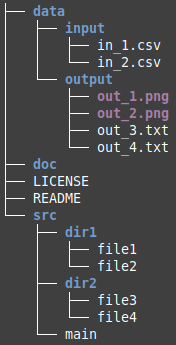
\includegraphics[width=4 cm]{figures/tree}
				\\
				Suggestion of working space
			\end{minipage}

		\subsection{Universal development rules}
			Each language has some specific mandatory rules. Yet there exists come common good practices:

			\subsubsection{Language}
                Code must be written in English language since:
				\begin{itemize}
					\setlength\itemsep{0pt}
					\item The syntax of the language is English.
					\item Scientific community communicates using English.
					\item Development problems are described in English on dedicated forums.
				\end{itemize}

			\subsubsection{Naming conventions}
				\begin{minipage}{0.75\textwidth}
					Some rules must be respected:
					\begin{itemize}
						\setlength\itemsep{0pt}

						\item In most of the languages, do not use any accentuation or special character.
						\item CamelCase or snake\_case \\
						Same everywhere in the code.
					\end{itemize}
				\end{minipage}
				\begin{minipage}{0.55\textwidth}
					\begin{tabular}{cc}
						& \begin{huge}
							  \textcolor{red}{camelCase}
						\end{huge} \\
						\\
						& \begin{huge}
							  \textcolor{red}{snake\_case}
						\end{huge} \\
						\\
						& \begin{huge}
							  \textcolor{red}{nocase}
						\end{huge}                               \\
					\end{tabular}
				\end{minipage}

				\paragraph{Variables} \mbox{}\\

					\begin{minipage}{0.45\textwidth}
							In the common case, a variable name must be:
							\begin{itemize}
								\setlength\itemsep{0pt}
								\item Short ($\leq$ 25 characters)
								\item Explicit
								\item Without any references to its type
								\item Using plural form if it's a container-like

							\end{itemize}
							Global variables are written \\ in
							UPPER\_SNAKE\_CASE.
							\\


					\end{minipage}
					\begin{minipage}{0.55\textwidth}
							\begin{tabular}{cc}
								\hline
								Incorrect    & Correct           \\
								\hline
								myvar                & dyn\_viscosity    \\
								a\_very\_long\_var   & input\_paths      \\
								temporaryArraySTRING & initialConditions

							\end{tabular}
					\end{minipage}
					In a software development process, an explicit variable name tells the user about the physical (or mathematical, etc \ldots) meaning
                    of the variable. Each wisely-defined variable name represents a lot of saved time when using the code as it is understood with less effort.
					lit le code.

				\paragraph{Functions and methods}  \mbox{}\\
					The name of a function:
					\begin{itemize}
							\item \textbf{Starts with a verb} à l'impératif at the imperativ form.
							\item Does not mention the type of input or output data.
					\end{itemize}

			\subsubsection{Indentation and spacing}
				Some languages have few constraints regarding indentation and spacing. In these cases:
				\begin{itemize}
					\setlength\itemsep{0pt}
					\item Do not exceed 100 characters as a length of code lines.
					\item Indent the same way instructions blocs that share the same structure, or let the IDE do it for you.
				\end{itemize}

			\subsubsection{Nested code}
				Nested code is difficult to read. For instance, do not nest multiple calls to functions in a one-liner as follows:
				\begin{verbatim}
							Float32 solar_power = compute_solar_power(get_area(solar_panel),
																	  get_irradiance(
																		             download_weather(get_actual_time())))
				\end{verbatim}
				Instead, write as many lines as needed:
				\begin{verbatim}
							Float32 solar_area = get_area(solar_panel)
                            Time current_time = get_actual_time()
							WeatherData Geneve_weather = download_weather(current_time)
							Float32 Geneve_irradiance = get_irradiance(Geneve_weather)
							Float32 solar_power = compute_solar_power(solar_area, Geneve_irradiance)
							delete(solar_area, Geneve_weather, Geneve_irradiance)               # optional in most languages
				\end{verbatim}


			\subsubsection{Comments}
                Comments start with a special character or set of characters that is defined for each language. Yet, 
                comment characters must not be inserted manually as:
				\begin{itemize}
					\setlength\itemsep{0pt}
					\item It is less readable (unwanted spaces at wrong places)
					\item It creates indentations error whenever you remove manually this comment sign
					\item Automatic removal by the IDE might not be possible
				\end{itemize}
                Instead, you must use the IDE shortcut for defining either line comments or block comments.


	\section{Comment and documentation}
		\label{sec:commenter}

		\subsection{Differences}
			A comment is a short explanation in the code that helps any \textbf{developer} to understand a few instructions. A comment may be only temporary.
            A commented code is mush simpler to understand. \\

			A documentation is an exhaustive explanation for the \textbf{user} of the code. The documented parts of the code are the one that constitute its API.

		\subsection{Comment a code}
			A comment must be inserted at least in the following cases:
			\begin{enumerate}
				\setlength\itemsep{0pt}
				\item \label{itm:fixme} Bug to be corrected
				\item \label{itm:todo} Local code improvement needed
				\item The way a difficult bug was solved
				Exemple:
				\begin{verbatim}
					UInt64 simulation_timestep = get_timestep()  // UInt64 prevents overflow
				\end{verbatim}
				\item Unusual instructions, ye tneeded.
				Exemple:
				\begin{verbatim}
					parse_request(parser=Parser.NO_DEFAULT, timeout=NULL) // default timeout (3 min) 
					                                                      // is too short
				\end{verbatim}
				\item Reference to a scientific article or an important scientific methodology or result
				Exemple:
				\begin{verbatim}
					Array[Float32] fourier_coefs = adapted_fourier_transform() //cf DOI 04.52/j.fake.206.1815
				\end{verbatim}
				This type of comments does not intend to replace an exhaustive scientific description of the code in a dedicated document.
				\item Some parameters are specified or a section of code is made unavailable (i.e.: "commented out")
				Exemple:
				\begin{verbatim}
					Int8 thermal_diffusivity = 9 // get_thermal_properties() has to be fixed
				\end{verbatim}
			\end{enumerate}

			Each IDE comes with specific keywords to make comments more readable. It is often the case of \textbf{fixme} (see \ref{itm:fixme}) and \textbf{todo} (see \ref{itm:todo}). \\

		\subsection{Document a code}

			\subsubsection{Content of a documentation}
				The documentation section of a function must give some information about the following points, from most to less important:
				\begin{enumerate}
					\label{enum:doc_content}
					\setlength\itemsep{0pt}
					\item What the function does  \label{enm:what}
					\item Input parameters
					\begin{itemize}
						\setlength\itemsep{0pt}
						\item types
						\item what they describe
						\item the set of expected values, if any
						\item the default value, if any
						\item physical unit, if any 
					\end{itemize}
					\item Same for output parameters \label{enm:out_params}
					\item Related functions 
					\item Detail of the operations achieved by the function
					\item Complete scientific references
					\item Use case examples of the function \label{enm:examples}
				\end{enumerate}
				\textbf{Points \ref{enm:what} to \ref{enm:out_params} are mandatory}.
				The other are optional yet recommended, in particular \ref{enm:examples}. \\
				Note that writting the documentation of a code is an iterative process: going through the entire code reveals some bug to fix, before going further into the documentation.

			\subsubsection{Documentation: howto}

				\paragraph{Documentation writing}
					The documentation is written into the code. It is often located:
					\begin{itemize}
							\setlength\itemsep{0pt}
							\item Either at the line before the function definition
							\item Or in the function body
					\end{itemize}
					A particular syntax is adoptéed to reference a component of the code (variable, function, \ldots) or the language (types, \ldots).

				\paragraph{Documentation generation}
					Each documentation block is then rendered in an easy-to-read format:
					\begin{itemize}
							\setlength\itemsep{0pt}
							\item HTML: if documentation is hosted on the web \url{https://about.readthedocs.com/}
							\item Latex/PDF: if documentation is shared locally
					\end{itemize}
					The built document is called the \textquote{API reference} because it makes it possible to entirely use the software according to its API.
					Some famous documentation builders are:
					\begin{itemize}
							\setlength\itemsep{0pt}
							\item Javadoc (Java)
							\item Doxygen (C, C++)
							\item Sphinx (Python)
					\end{itemize}

					\begin{figure}
							\centering
							\begin{tabular}{lr}
								\fbox{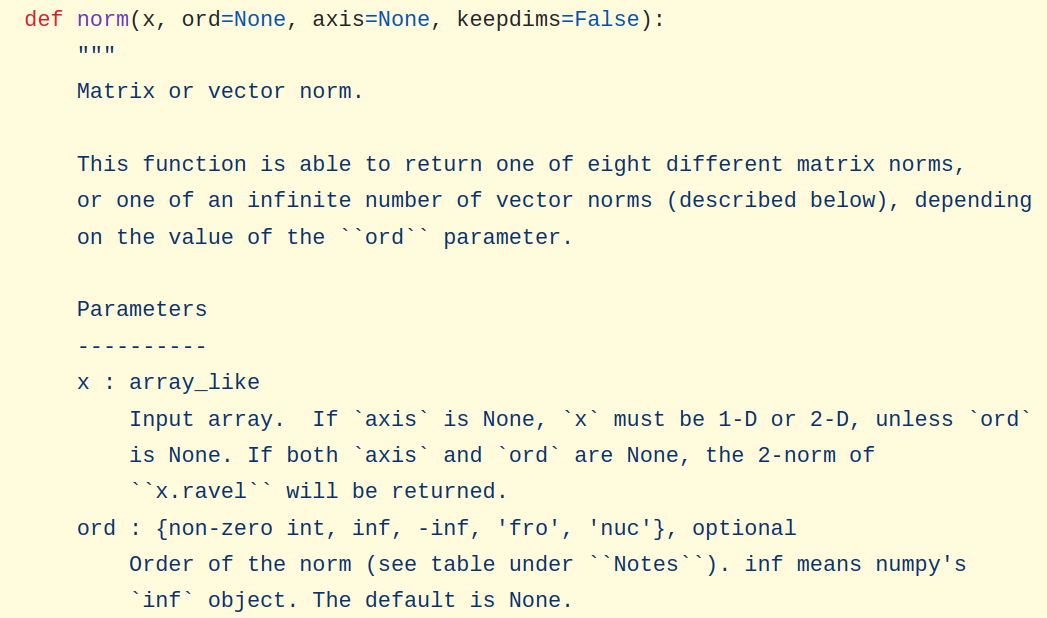
\includegraphics[height=5cm]{figures/doc_source.png}} &
								\fbox{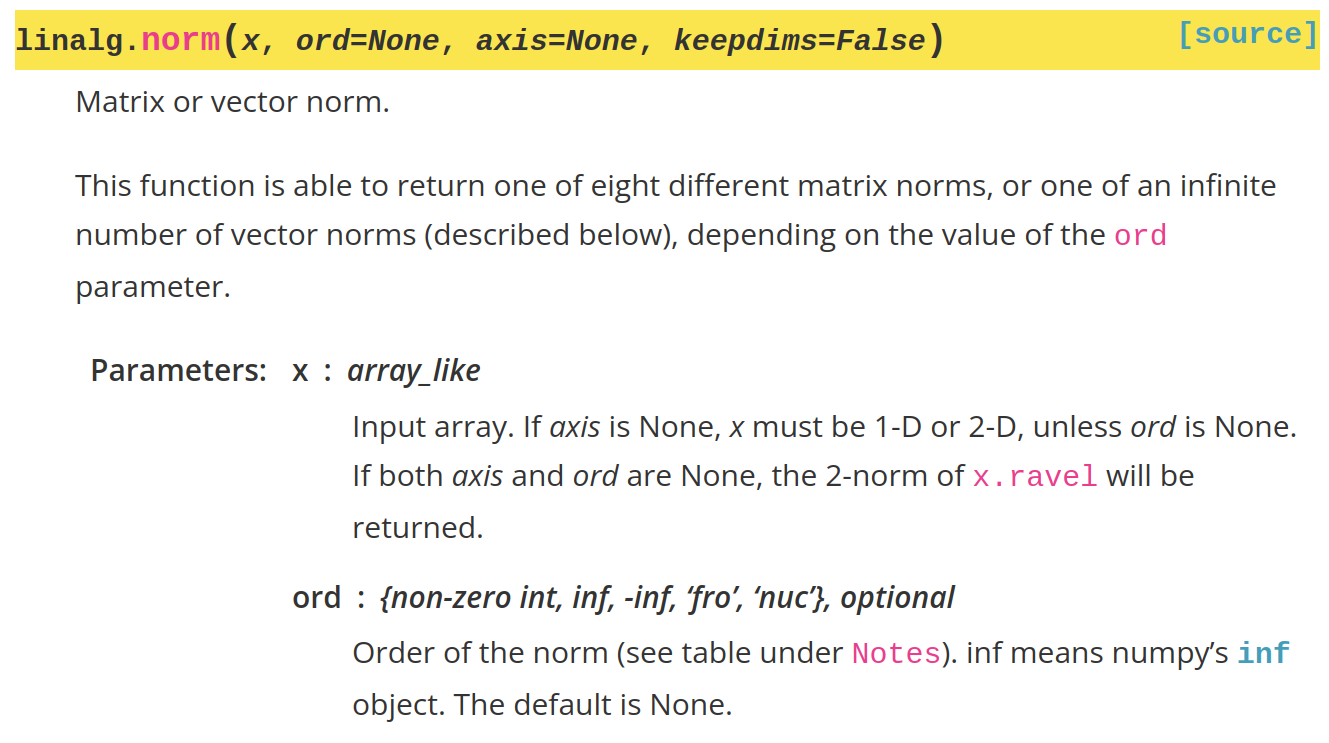
\includegraphics[height=5cm]{figures/doc_generated.png}}
							\end{tabular}
							\caption{Example of Python documentation: code side and HTML rendering. \\
							\scriptsize{(source: \url{https://numpydoc.readthedocs.io/en/latest/example.html}})}
							\label{fig:}
					\end{figure}
					Other than the API reference, the user can find on the web some special documentations to learn a programming language or a specific library:
					\begin{itemize}
							\setlength\itemsep{0pt}
							\item Getting started : suggestions of code and important concepts that cover most of development needs
							\item Tutorials: achieve very specific things with the tool you learn
					\end{itemize}

					\newpage


















	\section{Example}
		This part shows the different development steps applied to a fictive math problem (parts \ref{sec:cerner}, \ref{sec:dev}, \ref{sec:commenter})
		Let's solve the following differential equation:
		\begin{equation}
		(E)
			\quad \ddot{\theta} + w_0^2 \sin \theta = 0
			\label{eq:diff}
		\end{equation}
		Given:
		\begin{itemize}
			\setlength\itemsep{0pt}
			\item $\theta$ a time dependant function, with $t \in [0, 10]$
			\item initial conditions:
			\begin{align}
				\theta_0&=\theta(0)=\frac{\pi}{8}  \\
				\theta_0&=\theta'(0)=0
			\end{align}
			\item $w_0^2$  takes one of the following values:
			\begin{equation}
				w_0^2 \in \{0.05, 0.5, 5, 50, 500\}
			\end{equation}
		\end{itemize}

		\subsection{Identify one's problem}

			\subsubsection{Define the scientific goal}
				Our code must be able to:
				\begin{enumerate}
					\setlength\itemsep{0pt}
					\item Read a parameter file
					\item Solve a differential equation using the parameters specified by the file
					\item Plot and save a diagram presenting the solution to the equation
				\end{enumerate}

				A discretization on $t$ makes it possible to get a solution close to the formal one.
				Conversely, a formal resolution would be difficult with the $\sin$. \\

				The input data ($w_0^2$) is reliable since these are independant parameters of typical amplitude regarding this type of equations. \\

				The exactness of the result will be evaluated usng the approximation for small $\theta_0$ values:
				\begin{equation*}
					\theta: x \rightarrow \theta_0 \cos(w_0x)
				\end{equation*}

				This problem is deterministic, and we shall check we get the same solution from one run to another either graphically or numerically.

			\subsubsection{Choose the language}
				This problem does not represent a heavy CPU task. Yet, discretization and numerically stable solving both require a dedicated library.
				\textit{Julia} language is adaptated to analytic maths problems, using dedicated libraries such as 
                \textit{SciML} (solving) and \textit{Plots} (plotting). This language is a high-level language, hence dealing with data input/output will be easy.

			\subsubsection{Define a development plan}
				Table \ref{tab:planning_ex} is a suggestion of development plan. \\
                note: Parameters reading from the disk is not prioritary and could take place at the second step only.

				\begin{table}[h!]
					\scriptsize
					\centering
					\caption{Proposal of development plan: exercise}
					\begin{tabular}{|p{4cm}|p{6cm}|p{2cm}|}
						\hline
						\textbf{Step} & \textbf{Actions} & \textbf{Duration} \\
						\hline
						1. meet the the primary purpose of the code.
						&
						\textcolor{blue}{read and store parameters values} \newline
						Define and solve the equation. \newline
						Perform aquick draft plot of the solution.
						&
						1 hour
						\\
						\hline
						2. \textcolor{blue}{Structure the code}
						& Build an API. \newline
						Display some progress information for the user. \newline
						Customizz and save the results plot.
						& 1 hour
						\\
						\hline
						3. Optimize the code
						& Profile and analyse the running time. \newline
						Evaluate potential time savings. \newline
						Speed up the code.
						& 30 min \\
						\hline
						4. Document the code for your own interest
						& Description of every difficult instruction.
						& 10 min \\
						\hline
						5. Document the code for other users of the code
						& Write documentation block of each function. \newline
						Build as html.
						& 30 min \\

						\hline

					\end{tabular}
					\label{tab:planning_ex}
				\end{table}

		\subsection{Develop}

			\subsubsection{Preparation}

				\paragraph{Choose an IDE}
					Regarding Julia language, the largest community IDE is Visual Studio Code with the dedicated plugin.

				\paragraph{Organize your working space}
					\mbox{} \\
					\begin{minipage}{.55\textwidth}
							For instance, let's create 3 source files, one for each basic functionality. All of them are supervised by the file \textit{main.jl}. \\
							Yet, at step 1, (see Table \ref{tab:planning_ex}), all of the code is in \textit{main.jl}.
							Code structuration befins at step 2.
					\end{minipage}
					\begin{minipage}{.30\textwidth}
							\centering
							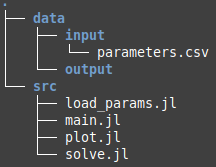
\includegraphics[width=4cm]{figures/diff_equation/working_dir_beginning}
							\\
							Actual structure of the working dir.

					\end{minipage}
					\newpage

			\subsubsection{Development}

				\paragraph{Step 1: meet the the primary purpose}
					Equation \ref{eq:diff} is transformed into 2 equations of first order:
					\begin{align*}
							\dot{\theta}(t) &= \omega(t) \\
							\dot{\omega}(t) &= - w_0^2 \theta(t)
					\end{align*}
					Let's call $u$ the result vector:
					\begin{equation*}
							u =
							\begin{bmatrix}
								\theta \\
								\omega
							\end{bmatrix}
					\end{equation*}
					Below, a first version of the code for step 1. \\
					\vspace{0.5cm}
					\mbox{} \\
					\begin{minipage}{0.65\textwidth}
							\centering
							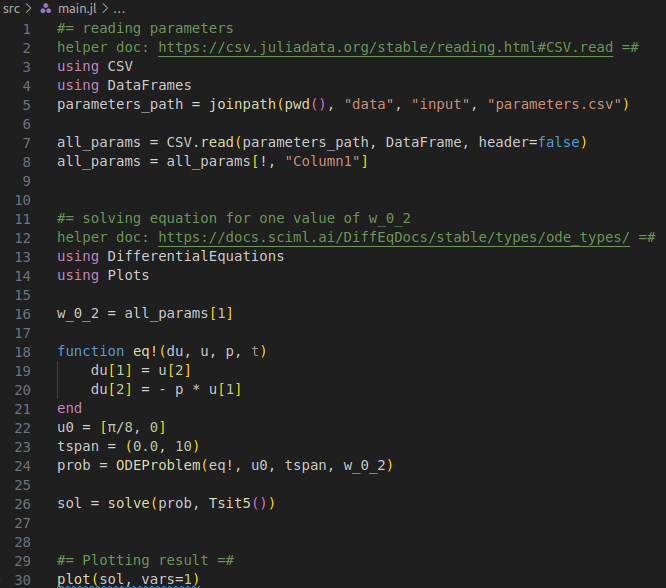
\includegraphics[width=11cm]{figures/diff_equation/code_step_1.png}
							\\
							Code - step 1
					\end{minipage}
					\begin{minipage}{0.35\textwidth}
							\centering
							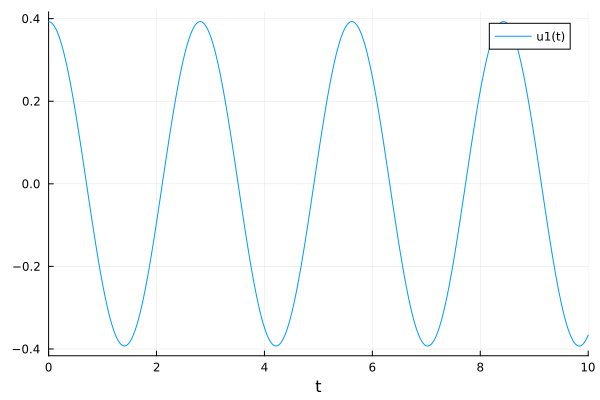
\includegraphics[width=7cm]{figures/diff_equation/plot_step_1.png}
							\\
							\quad $\theta$ as a function of time - step 1
					\end{minipage}

				\newpage
				\paragraph{Step 2: structure the code}
					The following taks are achieved:
					\begin{itemize}
							\setlength\itemsep{0pt}
							\item Split up of the code in dedicated files.
							\item Use of functions
							\item Check of parameters compliance
							\item Display of log messages
							\item Custom of the plot, disk save
					\end{itemize}
					See figures \ref{fig:step2_code} and \ref{fig:step2_plot}.
					\begin{figure}[h!]
							\centering
							\caption{Code - step 2}
%					    \label{tab:}
							\begin{tabular}{cc}
								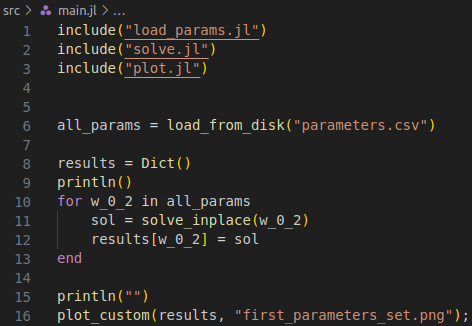
\includegraphics[width=7.5cm]{figures/diff_equation/code_main_step_2.png}
								&
								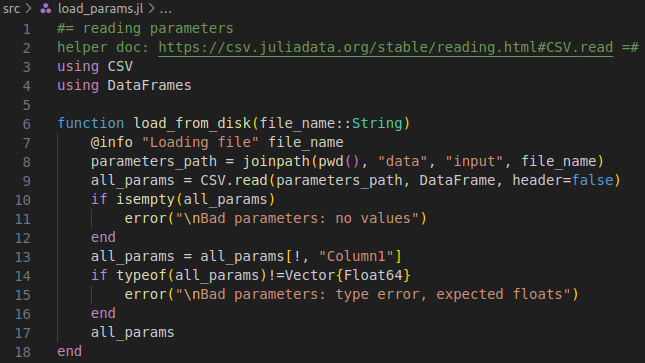
\includegraphics[width=7.5cm]{figures/diff_equation/code_load_params_step_2} \\
								\textit{main.jl}
								&
								\textit{load\_params.jl} \\
								\\
								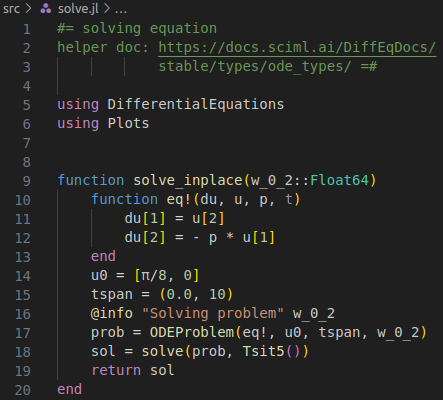
\includegraphics[width=7.5cm]{figures/diff_equation/code_solve_step_2}
								&
								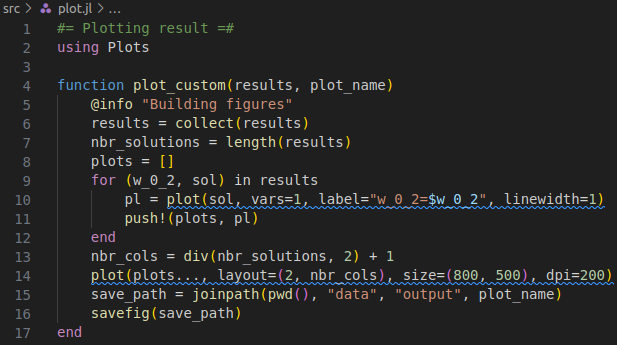
\includegraphics[width=7.5cm]{figures/diff_equation/code_plot_step_2} \\
								\textit{solve.jl}
								&
								\textit{plot.jl} \\
							\end{tabular}
							\label{fig:step2_code}
					\end{figure}
					\begin{figure}[h!]
							\centering
							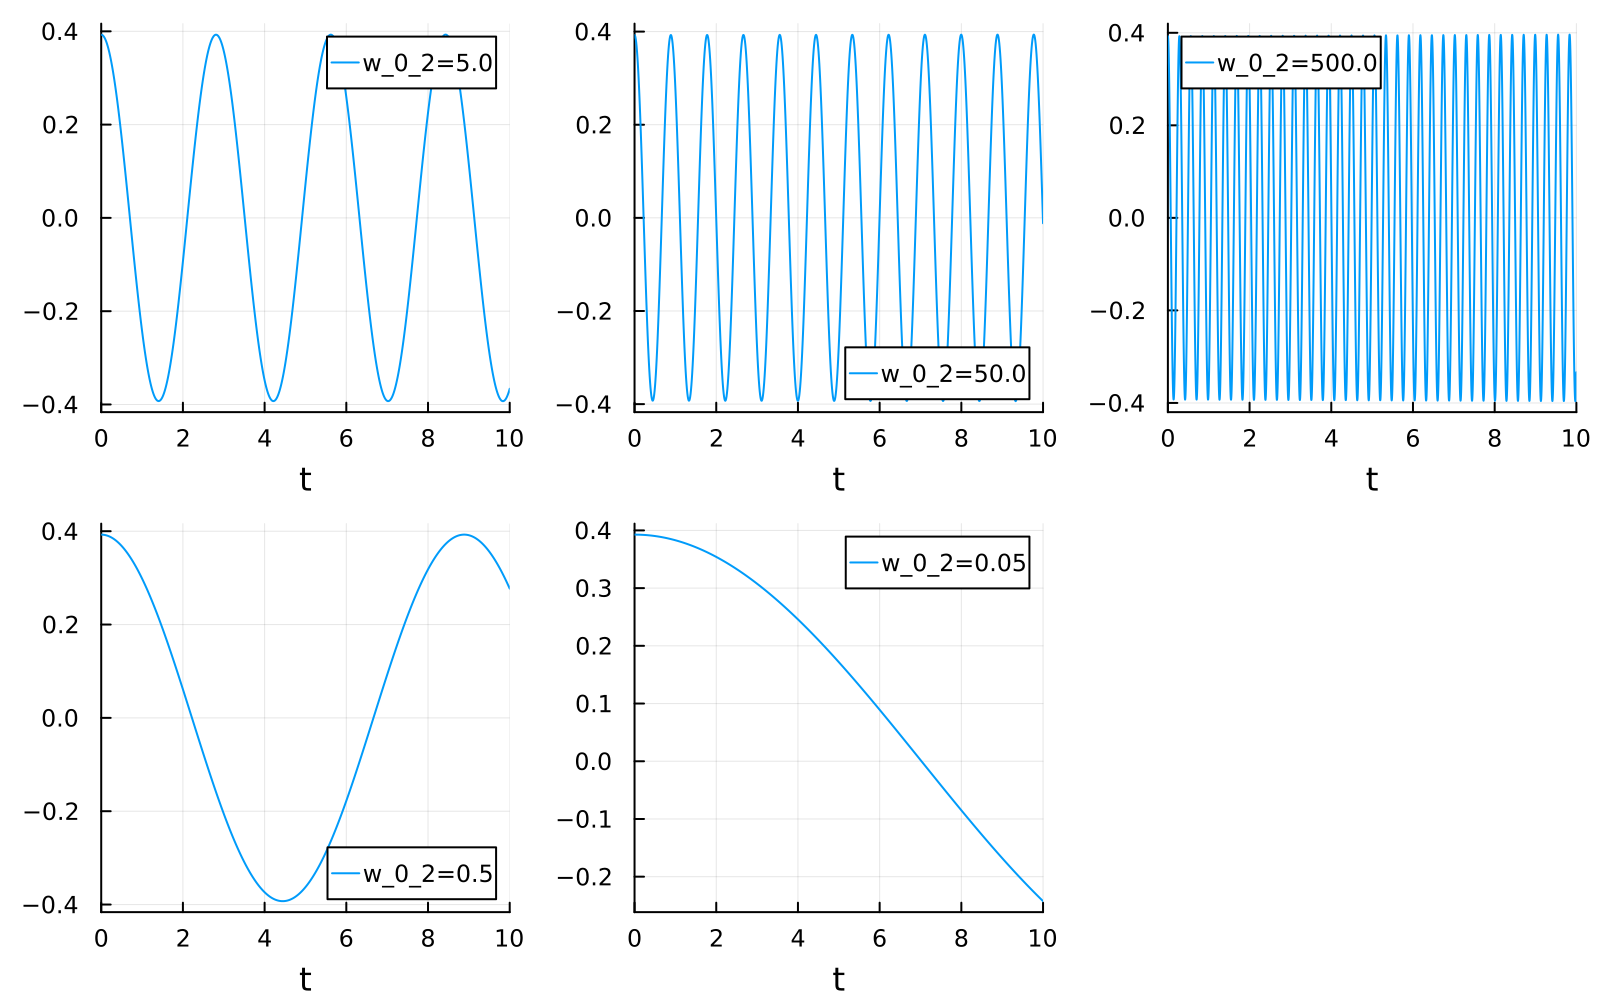
\includegraphics[width=14cm]{figures/diff_equation/first_parameters_set.png}
							\caption{Visualization - step 2}
							\label{fig:step2_plot}
					\end{figure}

				\newpage
				\paragraph{Step 3: optimize the code}

					\subparagraph{Measure the running time: overview} \mbox{} \\
						Every language, IDE and operating system comes with \textbf{benchmarking and profiling tools}.
						For this problem, the macro \textit{@benchmark} is used. it returns a total execution duration and an estimation of memory usage.
						\begin{center}
									\includegraphics[width=15cm]{figures/diff_equation/benchmark - étape 3.png}
						\end{center}
						Results:
						\begin{enumerate}
									\item On average, the code runs takes 0.36s to run and uses 14 MiB of memory (\textit{MiB=mebibyte}) \\
									\textrightarrow \quad \textbf{Is-it too much?}
									\item The standard deviation of running time is low.
						\end{enumerate}

					\subparagraph{Profile the running time} \mbox{} \\
						The macro \textit{@profile} makes it possible to focus on time consuming sections of the code.
						Figure \ref{fig:profile} shows a \textit{FlameGraph} of this analysis.
						\begin{figure}
									\centering
									\includegraphics[width=15cm]{figures/diff_equation/profile - étape 3}
									\caption{Running time decomposition}
									\label{fig:profile}
						\end{figure}

						Most of the running time comes from plotting and saving the results.
						This is an important part of the code that must be sped up. Two choices: \\
						\begin{minipage}{.5\textwidth}
									\begin{enumerate}
										\item Specify some variable types to speed up code interpretation.
										\begin{itemize}
											\item This is specific to Julia language
											\item Saved time: 15\%.
											\item \textbf{does not alter functionalities of the code}.
										\end{itemize}

										\item Do not save the plot on disk.
										\begin{itemize}
											\item Saved time: 30\%.
											\item \textbf{is a degradation of functionalities}.
										\end{itemize}
									\end{enumerate}
						\end{minipage}
						\begin{minipage}{1cm}
									\mbox{}
						\end{minipage}
						\begin{minipage}{.45\textwidth}
									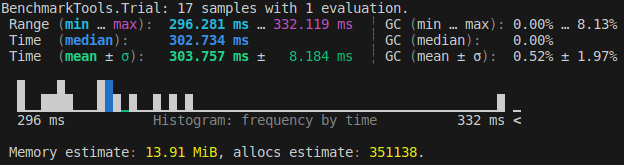
\includegraphics[width=9cm]{figures/diff_equation/benchmark - improved types - step 3} \\
									\mbox{} \\
									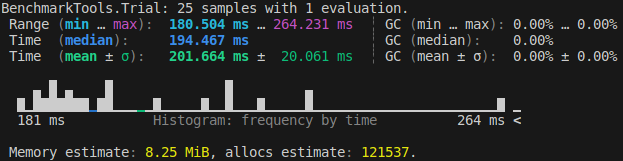
\includegraphics[width=9cm]{figures/diff_equation/benchmark - no_disk_write - step 3}
						\end{minipage}

				\paragraph{Step 4: document the code for your own interest}
                    Will be seen on a Python case.

				\paragraph{Step 5: document the code for other users of the code}
					Will be seen on a Python case.

\end{document}
